\documentclass[10pt,twocolumn]{article}

\usepackage[margin=0.68in,columnsep=0.22in]{geometry}
\usepackage[T1]{fontenc}
\usepackage[utf8]{inputenc}
\usepackage{lmodern}
\usepackage{microtype}
\usepackage{amsmath,amssymb}
\usepackage{graphicx}
\usepackage{booktabs}
\usepackage{algorithm}
\usepackage{algpseudocode}
\usepackage{tikz}
\usetikzlibrary{arrows.meta,positioning,shapes.geometric,calc}
\usepackage{pgfplots}
\usepackage{pgfplotstable}
\pgfplotsset{compat=1.18}
\usepackage{xcolor}
\usepackage[hidelinks]{hyperref}

\definecolor{accentblue}{HTML}{1D4ED8}
\definecolor{accentred}{HTML}{BE123C}
\definecolor{accentteal}{HTML}{0F766E}
\definecolor{slatebg}{HTML}{F8FAFC}

\title{\textbf{Decentralized Collective Evasion: Foundations of Swarm Intelligence and a Real-Time C++20 Interactive Demonstrator}}
\author{Prasad Desale \\ \small Under the guidance of Prof.\ K.\ K.\ Deshmukh \\ \small Source Code: \href{https://github.com/Pras2005/swarm-evader}{\texttt{https://github.com/Pras2005/swarm-evader}}}
\date{November 2026}

\begin{document}

\maketitle

\begin{abstract}
Swarm Intelligence (SI) investigates how coherent, adaptive macro-level behavior emerges from decentralized networks of simple agents interacting exclusively through local rules. This report presents both a theoretical synthesis of SI principles and the design, implementation, and empirical evaluation of \emph{Swarm Evader}---a lightweight, high-performance interactive demonstrator and game implemented in C++20 over a zero-dependency X11 software framebuffer. In the system, a user-controlled predator point navigates a continuous 2D arena while an autonomous flock of self-propelled agents (boids) coordinates via local cohesion, alignment, and separation rules augmented with smooth inverse-distance threat avoidance and shockwave dispersion. To sustain real-time frame rates for thousands of agents, neighbor queries are accelerated using a zero-allocation linked-list uniform spatial hash grid. Headless empirical benchmarks demonstrate a $5.21\times$ speedup at $N = 4{,}000$ agents over naive $O(N^2)$ search ($4.11\,\text{ms}$ vs.\ $21.39\,\text{ms}$ per step), while time-series and parameter-sweep experiments quantify predator-induced depolarization, selfish-herd compaction, and a monotonic reduction in predator capture rate from $61$ to $5$ tags as avoidance weight increases from $0.0$ to $8.5$.
\end{abstract}

\section{Introduction}
Across biological systems---from starling murmurations and schooling herring to foraging ant colonies---large collectives routinely solve complex spatial coordination and survival problems without a central planner or global state awareness~\cite{bonabeau1999swarm}. Each individual operates using strictly local sensory cues and rudimentary behavioral rules, yet the aggregate exhibits robustness, scalability, and rapid collective adaptation to external threats. In computer science and control theory, this phenomenon is formalized as \emph{Swarm Intelligence} (SI).

Interactive visual demonstrators play a critical pedagogical and diagnostic role in SI research: they expose how subtle parameter shifts in local interaction radii or steering weights produce qualitative phase transitions at the macroscopic scale. However, naive implementations that check all $N(N-1)$ agent pairs degrade quadratically, constraining interactive exploration to small populations.

This project develops \emph{Swarm Evader}, a self-contained C++20 demonstrator and interactive tag-evasion game in which the human user controls a mobile repulsor (predator) point via mouse or keyboard while an autonomous swarm dynamically fragments, flanks, compacts, and reforms to evade capture. The contributions of this work are threefold:
\begin{enumerate}
    \item A unified synthesis of SI foundations, contrasting spatial collective motion models with swarm optimization metaheuristics.
    \item A clean, zero-external-toolkit C++20 simulation and X11 rendering engine featuring a flat-array uniform spatial hash grid and deterministic verification tests.
    \item Empirical benchmarks analyzing computational scaling, collective order parameters under predation, and avoidance-weight sensitivity.
\end{enumerate}

\section{Foundations of Swarm Intelligence}

\subsection{Core Principles}
Bonabeau, Dorigo, and Theraulaz~\cite{bonabeau1999swarm} characterize swarm-intelligent systems through five foundational properties:
\begin{itemize}
    \item \textbf{Proximity:} Agents perform elementary spatial and temporal computations within bounded neighborhoods.
    \item \textbf{Quality:} The collective responds to environmental quality factors (e.g., threat gradients or resource density).
    \item \textbf{Diverse Response:} Individuals avoid committing all effort along a single channel, preserving adaptability under perturbation.
    \item \textbf{Stability:} The swarm does not radically alter its organizational mode for every minor environmental fluctuation.
    \item \textbf{Adaptability:} When the payoff outweighs switching cost, the collective rapidly transitions between behavioral regimes (e.g., cruising vs.\ evasive splitting).
\end{itemize}
Crucially, SI relies on \emph{decentralization}: removing or perturbing any subset of agents does not halt system operation, yielding graceful degradation.

\subsection{Taxonomy of Swarm Models}
Swarm intelligence spans two complementary research branches:

\paragraph{Metaheuristic Optimization.} Algorithms such as Ant Colony Optimization (ACO)~\cite{dorigo1996ant} and Particle Swarm Optimization (PSO)~\cite{kennedy1995particle} embed agents in abstract combinatorial or continuous objective landscapes. In ACO, agents communicate indirectly via \emph{stigmergy}---depositing and evaporating virtual pheromone trails along graph edges. In PSO, each particle updates its velocity toward both its personal historical best position and the global or topological neighborhood best.

\paragraph{Spatial Collective Motion.} Physical and behavioral models focus on coordinated kinematics in Euclidean space. Reynolds' seminal \emph{Boids} model~\cite{reynolds1987flocks} introduced three local steering behaviors---separation, alignment, and cohesion---capable of producing realistic flocking without scripted paths. Vicsek et al.~\cite{vicsek1995novel} simplified the system to constant-speed self-propelled particles with noisy alignment, establishing a kinetic phase transition from disordered gas-like motion to ordered collective flow as density increases or noise decreases. Couzin et al.~\cite{couzin2002collective} further organized interactions into concentric behavioral zones (repulsion, orientation, attraction) that explain transitions between swarming, toroidal milling, and polarized schooling. Olfati-Saber~\cite{olfati2006flocking} later provided formal Lyapunov stability guarantees for multi-agent flocking networks using $\alpha$-lattice potential fields and velocity consensus.

\subsection{Collective Evasion Under Predation}
When a predator enters a cohesive group, local threat-avoidance forces compete with alignment and cohesion. Biological and theoretical studies identify several emergent defense signatures:
\begin{itemize}
    \item \textbf{Selfish-Herd Compaction:} Agents on the exposed periphery steer inward or radially away, temporarily reducing nearest-neighbor spacing~\cite{hamilton1971geometry}.
    \item \textbf{Flash Expansion and Fountain Effect:} High-urgency radial repulsion splits the flock around the predator's trajectory, after which cohesion reunites the sub-flocks behind the threat.
    \item \textbf{Trafalgar Effect:} Because neighbors align with fleeing peers, evasive waves propagate outward faster than the predator's approach speed, alerting agents outside direct predator perception.
\end{itemize}
\emph{Swarm Evader} directly reproduces all three phenomena in real time.

\section{Mathematical Model of \emph{Swarm Evader}}

\subsection{Agent Kinematics}
Let the simulation domain be a bounded 2D arena $\Omega = [0, W] \times [0, H]$ with $W = 1280\,\text{px}$ and $H = 800\,\text{px}$. Each boid $i \in \{1,\dots,N\}$ maintains position $\mathbf{x}_i(t) \in \mathbb{R}^2$ and velocity $\mathbf{v}_i(t) \in \mathbb{R}^2$. Over discrete time step $\Delta t$, state evolution follows semi-implicit Euler integration with steering saturation:
\begin{align}
    \mathbf{v}_i^{\,\text{raw}}(t + \Delta t) &= \mathbf{v}_i(t) + \mathbf{a}_i(t)\,\Delta t, \\
    \mathbf{v}_i(t + \Delta t) &= \operatorname{clamp\_mag}\!\left(\mathbf{v}_i^{\,\text{raw}},\, v_{\min},\, v_{\max}\right), \\
    \mathbf{x}_i(t + \Delta t) &= \mathbf{x}_i(t) + \mathbf{v}_i(t + \Delta t)\,\Delta t,
\end{align}
where $\operatorname{clamp\_mag}(\mathbf{u}, v_{\min}, v_{\max})$ scales $\mathbf{u}$ so its Euclidean norm satisfies $\|\mathbf{v}_i\| \in [v_{\min}, v_{\max}]$ (default $v_{\min} = 85$, $v_{\max} = 270\,\text{px/s}$). Every steering term $\mathbf{s}$ is bounded by $\operatorname{limit}(\mathbf{s}, F_{\max})$ with $F_{\max} = 460\,\text{px/s}^2$, preventing numerical overshoot.

\subsection{Local Steering Forces}
Define the perception neighborhood $\mathcal{N}_i$ and separation neighborhood $\mathcal{S}_i$ of boid $i$ as:
\begin{align}
    \mathcal{N}_i &= \left\{ j \neq i : \|\mathbf{x}_j - \mathbf{x}_i\| \le R_{\text{perc}} \right\}, \\
    \mathcal{S}_i &= \left\{ j \neq i : 0 < \|\mathbf{x}_j - \mathbf{x}_i\| < R_{\text{sep}} \right\},
\end{align}
with default radii $R_{\text{perc}} = 56\,\text{px}$ and $R_{\text{sep}} = 24\,\text{px}$. Using Reynolds' desired-velocity steering operator $\Psi(\mathbf{d}, \mathbf{v}_i) = \operatorname{limit}\!\left(v_{\max}\hat{\mathbf{d}} - \mathbf{v}_i, F_{\max}\right)$ where $\hat{\mathbf{d}} = \mathbf{d}/\|\mathbf{d}\|$, the three canonical flocking forces are:
\begin{align}
    \mathbf{f}_{\text{coh}, i} &= \Psi\!\left(\frac{1}{|\mathcal{N}_i|}\sum_{j \in \mathcal{N}_i} \mathbf{x}_j - \mathbf{x}_i,\; \mathbf{v}_i\right), \\
    \mathbf{f}_{\text{align}, i} &= \Psi\!\left(\frac{1}{|\mathcal{N}_i|}\sum_{j \in \mathcal{N}_i} \mathbf{v}_j,\; \mathbf{v}_i\right), \\
    \mathbf{f}_{\text{sep}, i} &= \Psi\!\left(\sum_{j \in \mathcal{S}_i} \frac{\mathbf{x}_i - \mathbf{x}_j}{d_{ij}}\left(1 - \frac{d_{ij}}{R_{\text{sep}}}\right),\; \mathbf{v}_i\right),
\end{align}
where $d_{ij} = \|\mathbf{x}_i - \mathbf{x}_j\|$. Weighting separation inversely by proximity eliminates overlap singularities while gently spacing agents at equilibrium.

\subsection{Predator Avoidance, Pulse, and Containment}
Let $\mathbf{x}_P(t)$ denote the user-controlled predator point and $d_i = \|\mathbf{x}_i - \mathbf{x}_P\|$. Within threat radius $R_P = 165\,\text{px}$, normalized proximity $\xi_i = 1 - d_i / R_P \in (0, 1]$ drives a nonlinear urgency gain $u(\xi_i) = \xi_i (0.4 + 1.6\xi_i)$:
\begin{equation}
    \mathbf{f}_{\text{avoid}, i} =
    \begin{cases}
        u(\xi_i)\,\operatorname{limit}\!\left(v_{\max}\hat{\mathbf{r}}_{iP} - \mathbf{v}_i,\, 1.4 F_{\max}\right), & d_i < R_P, \\
        \mathbf{0}, & d_i \ge R_P,
    \end{cases}
\end{equation}
where $\hat{\mathbf{r}}_{iP} = (\mathbf{x}_i - \mathbf{x}_P)/d_i$ is the outward unit vector. In interactive \emph{Attract} mode, the target direction reverses toward $\mathbf{x}_P$ with gain $0.65\,u(\xi_i)$, producing swirling orbital swarms. Additionally, triggering a shockwave pulse at $\mathbf{x}_{\text{pulse}}$ emits an expanding ring of radius $r_{\text{wave}}(\tau) = R_{\text{pulse}}\tau$ ($\tau \in [0,1]$, $R_{\text{pulse}} = 275\,\text{px}$, band $\beta = 65\,\text{px}$) exerting radial impulse $\mathbf{f}_{\text{pulse}, i}$ proportional to $(1 - |\|\mathbf{x}_i - \mathbf{x}_{\text{pulse}}\| - r_{\text{wave}}|/\beta)$.

Soft wall containment $\mathbf{f}_{\text{bound}, i}$ applies linear inward steering whenever $\mathbf{x}_i$ enters a boundary margin $m = 65\,\text{px}$ along any edge of $\Omega$. The total acceleration is then the weighted superposition:
\begin{equation}
\begin{aligned}
    \mathbf{a}_i =\;& w_c \mathbf{f}_{\text{coh}, i} + w_a \mathbf{f}_{\text{align}, i} + w_s \mathbf{f}_{\text{sep}, i} \\
                    & + w_p \mathbf{f}_{\text{avoid}, i} + w_b \mathbf{f}_{\text{bound}, i} + \mathbf{f}_{\text{pulse}, i},
\end{aligned}
\end{equation}
with default weights $(w_c, w_a, w_s, w_p, w_b) = (1.00, 1.25, 1.85, 4.80, 3.50)$. Figure~\ref{fig:forces} illustrates the local geometry around a focal boid.

\begin{figure}[t]
\centering
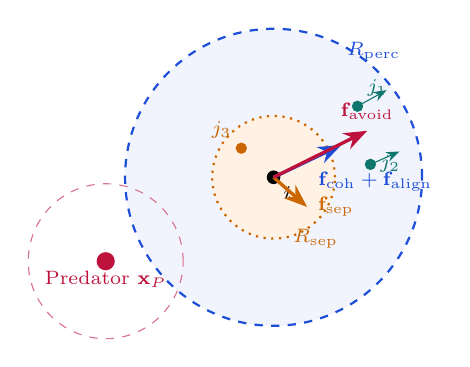
\begin{tikzpicture}[scale=0.82, >=Stealth]
    % Perception and separation zones
    \fill[accentblue!6] (0,0) circle (2.3);
    \draw[dashed, accentblue, thick] (0,0) circle (2.3);
    \fill[orange!10] (0,0) circle (0.95);
    \draw[dotted, orange!80!black, thick] (0,0) circle (0.95);

    % Labels for radii
    \node[accentblue, font=\scriptsize] at (1.55, 1.95) {$R_{\text{perc}}$};
    \node[orange!80!black, font=\scriptsize] at (0.65, -0.95) {$R_{\text{sep}}$};

    % Neighbor boids
    \fill[accentteal] (1.3, 1.1) circle (2.5pt) node[above right, font=\scriptsize] {$j_1$};
    \draw[->, accentteal, thin] (1.3, 1.1) -- ++(0.45, 0.25);

    \fill[accentteal] (1.5, 0.2) circle (2.5pt) node[right, font=\scriptsize] {$j_2$};
    \draw[->, accentteal, thin] (1.5, 0.2) -- ++(0.45, 0.2);

    \fill[orange!80!black] (-0.5, 0.45) circle (2.5pt) node[above left, font=\scriptsize] {$j_3$};

    % Predator
    \fill[accentred] (-2.6, -1.3) circle (4pt) node[below, font=\scriptsize] {Predator $\mathbf{x}_P$};
    \draw[dashed, accentred!60] (-2.6, -1.3) circle (1.2);

    % Focal boid
    \fill[black] (0,0) circle (3pt) node[below right, font=\scriptsize] {$i$};

    % Force vectors
    \draw[->, very thick, accentblue] (0,0) -- (1.05, 0.50) node[midway, below right, font=\scriptsize] {$\mathbf{f}_{\text{coh}}+\mathbf{f}_{\text{align}}$};
    \draw[->, very thick, orange!80!black] (0,0) -- (0.52, -0.46) node[right, font=\scriptsize] {$\mathbf{f}_{\text{sep}}$};
    \draw[->, very thick, accentred] (0,0) -- (1.45, 0.72) node[above, font=\scriptsize] {$\mathbf{f}_{\text{avoid}}$};
\end{tikzpicture}
\caption{Local interaction geometry around focal boid $i$. Neighbors inside $R_{\text{perc}}$ contribute cohesion and alignment, close neighbors inside $R_{\text{sep}}$ trigger separation, and the predator point $\mathbf{x}_P$ induces high-urgency avoidance.}
\label{fig:forces}
\end{figure}

\subsection{Collective Order Parameters}
To quantify emergent swarm state without subjective visual inspection, the simulator computes three real-time observables each step:
\begin{enumerate}
    \item \textbf{Polarization}~\cite{vicsek1995novel,couzin2002collective}:
    \begin{equation}
        \Phi(t) = \frac{1}{N} \left\| \sum_{i=1}^N \frac{\mathbf{v}_i(t)}{\|\mathbf{v}_i(t)\|} \right\| \in [0, 1],
    \end{equation}
    measuring global directional alignment ($\Phi \approx 1$ for unified schooling, $\Phi \approx 0$ for isotropic or symmetrically split motion).
    \item \textbf{Mean Nearest-Neighbor Distance} $\bar{d}_{\text{NN}}(t)$ across agents with non-empty $\mathcal{N}_i$, capturing spatial compaction under predation.
    \item \textbf{Panic Fraction} $\rho_{\text{panic}}(t)$, the proportion of agents whose smoothed threat level exceeds $0.25$, alongside predator capture score (tags within $R_{\text{cap}} = 15\,\text{px}$).
\end{enumerate}

\section{System Architecture \& Spatial Hashing}

\subsection{Software Design}
\emph{Swarm Evader} is written in modular C++20 and compiled with \texttt{g++ -O3}. Rather than relying on heavy external game engines, graphics are rendered directly into a 32-bit \texttt{framebuffer\_} array blitted to an X11 window via \texttt{XPutImage}. This guarantees portability across minimal Linux environments while supporting alpha-blended perception rings, directional boid chevrons with motion trails, a custom $5\times 7$ bitmap HUD font, and live parameter controls (mouse/WASD movement, pulse shockwave, attract/repel toggle, live $N$ scaling, presets, and spatial grid debug overlay). Figure~\ref{fig:arch} summarizes the system pipeline, and Figure~\ref{fig:screenshots} presents live screenshots of both predator-evasion mode and the spatial-hashing debug overlay.

\begin{figure*}[t]
\centering
\begin{minipage}[t]{0.49\textwidth}
    \centering
    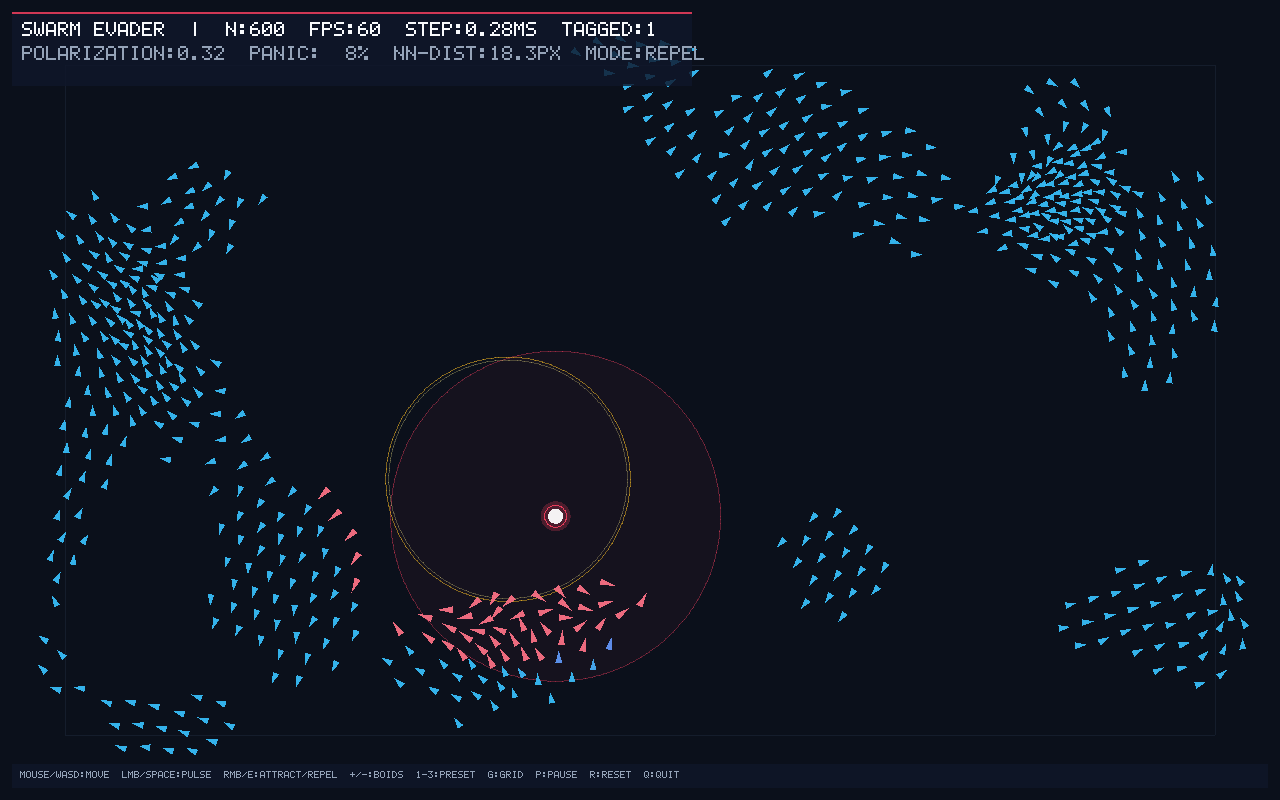
\includegraphics[width=\linewidth]{figures/shot_evasion.png}
    \vspace{2pt}
    {\footnotesize (a) Active predator evasion with shockwave pulse and panic coloring.}
\end{minipage}
\hfill
\begin{minipage}[t]{0.49\textwidth}
    \centering
    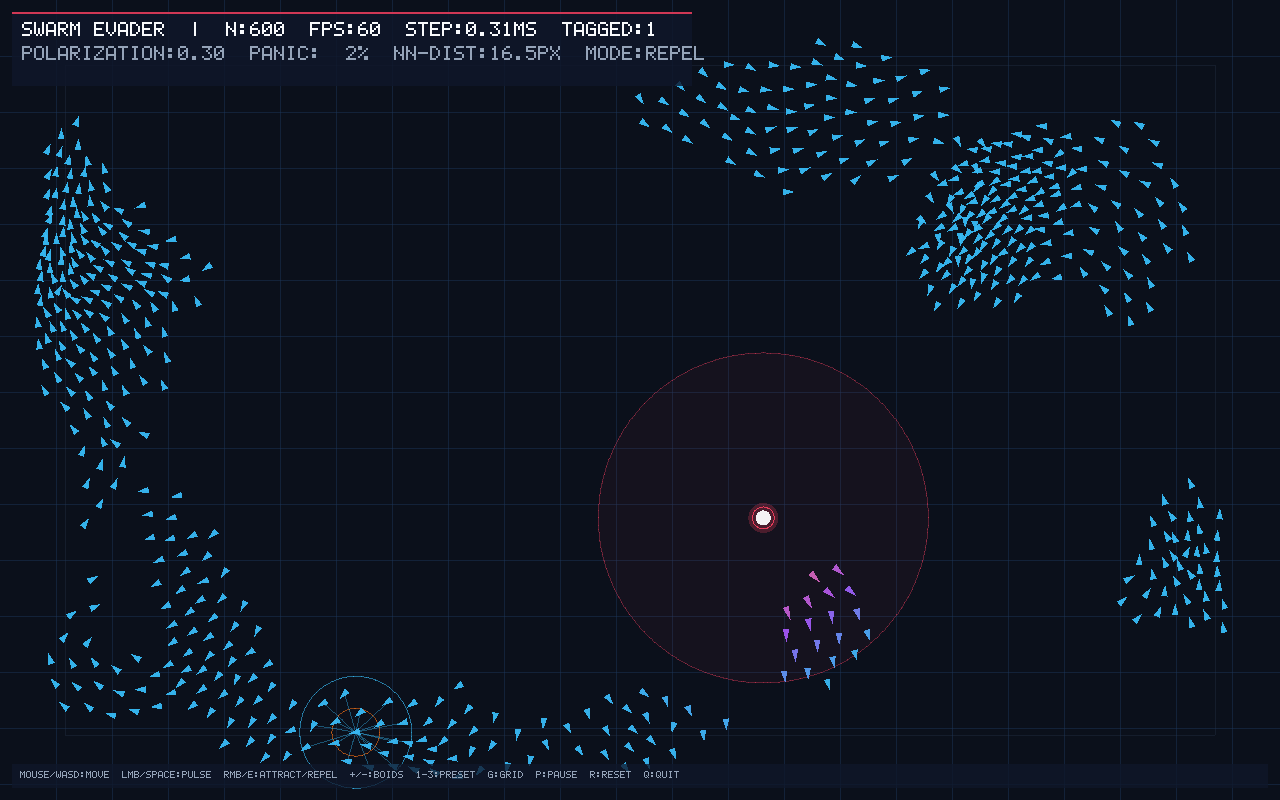
\includegraphics[width=\linewidth]{figures/shot_debug.png}
    \vspace{2pt}
    {\footnotesize (b) Spatial hash grid overlay (\texttt{G}), showing $R_{\text{perc}}$, $R_{\text{sep}}$, and neighbor links.}
\end{minipage}
\caption{Live captures from the \emph{Swarm Evader} X11 framebuffer ($N=600$, $1280\times 800$ arena). Calm boids appear in cyan, transitioning smoothly through violet to coral-red as threat urgency increases near the predator's danger radius.}
\label{fig:screenshots}
\end{figure*}

\begin{figure}[t]
\centering
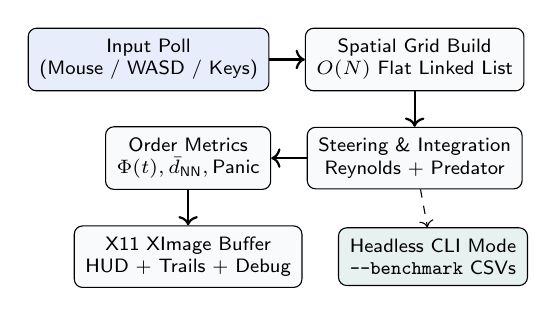
\begin{tikzpicture}[
    node distance=0.45cm and 0.45cm,
    box/.style={draw, rounded corners=3pt, fill=slatebg, minimum height=0.72cm, align=center, font=\scriptsize\sffamily, inner sep=4pt}
]
    \node[box, fill=accentblue!10] (input) {Input Poll\\(Mouse / WASD / Keys)};
    \node[box, right=of input] (grid) {Spatial Grid Build\\$O(N)$ Flat Linked List};
    \node[box, below=of grid] (force) {Steering \& Integration\\Reynolds + Predator};
    \node[box, left=of force] (metrics) {Order Metrics\\$\Phi(t), \bar{d}_{\text{NN}}, \text{Panic}$};
    \node[box, below=of metrics, minimum width=2.4cm] (render) {X11 XImage Buffer\\HUD + Trails + Debug};
    \node[box, right=of render, minimum width=2.4cm, fill=accentteal!10] (bench) {Headless CLI Mode\\\texttt{{-}{-}benchmark} CSVs};

    \draw[->, thick] (input) -- (grid);
    \draw[->, thick] (grid) -- (force);
    \draw[->, thick] (force) -- (metrics);
    \draw[->, thick] (metrics) -- (render);
    \draw[->, dashed] (force) -- (bench);
\end{tikzpicture}
\caption{Modular architecture of \emph{Swarm Evader}, sharing a single deterministic physics core across the interactive X11 loop, unit test suite, and headless benchmark driver.}
\label{fig:arch}
\end{figure}

\subsection{Zero-Allocation Uniform Spatial Hash Grid}
An all-pairs neighbor search evaluates $N(N-1)$ Euclidean distances per step ($O(N^2)$). Because boid perception is strictly bounded by $R_{\text{perc}}$, we partition $\Omega$ into square cells of side $c = R_{\text{perc}}$, creating $C = \lceil W/c \rceil$ columns and $R = \lceil H/c \rceil$ rows. Instead of allocating a \texttt{std::vector<int>} per cell each frame, we store two contiguous flat arrays: \texttt{cellHeads} of size $C \cdot R$ and \texttt{next} of size $N$, forming intrusive linked lists in pre-allocated memory (Algorithm~\ref{alg:grid}).

\begin{algorithm}[t]
\caption{Zero-Allocation Spatial Grid Build \& Query}
\label{alg:grid}
\begin{algorithmic}[1]
\State \textbf{Build:} Fill \texttt{cellHeads}$[0 \dots CR-1] \gets -1$
\For{$i = 0$ \textbf{to} $N - 1$}
    \State $c_x \gets \operatorname{clamp}(\lfloor x_i / c \rfloor, 0, C - 1)$
    \State $c_y \gets \operatorname{clamp}(\lfloor y_i / c \rfloor, 0, R - 1)$
    \State $k \gets c_y C + c_x$
    \State \texttt{next}$[i] \gets$ \texttt{cellHeads}$[k]$; \quad \texttt{cellHeads}$[k] \gets i$
\EndFor
\State \textbf{Query}($i$): Inspect $3 \times 3$ stencil $(c_x + \delta_x, c_y + \delta_y)$ for $\delta_x, \delta_y \in \{-1, 0, 1\}$
\ForAll{valid cell $k'$}
    \State $j \gets$ \texttt{cellHeads}$[k']$
    \While{$j \neq -1$}
        \If{$j \neq i$ \textbf{and} $\|\mathbf{x}_j - \mathbf{x}_i\|^2 \le R_{\text{perc}}^2$}
            \State Accumulate cohesion, alignment, separation
        \EndIf
        \State $j \gets$ \texttt{next}$[j]$
    \EndWhile
\EndFor
\end{algorithmic}
\end{algorithm}

Because $c = R_{\text{perc}}$, any neighbor within Euclidean distance $R_{\text{perc}}$ must reside in the agent's own cell or one of its 8 immediate Moore neighbors. For constant spatial density $\rho = N / (WH)$, the expected number of candidates inspected per agent is $\bar{m} \approx 9\rho R_{\text{perc}}^2 = O(1)$, reducing total frame complexity from $O(N^2)$ to $O(N)$. When $N$ increases inside a \emph{fixed} arena area $WH$, $\rho$ grows linearly with $N$, so candidate work scales as $O(9 R_{\text{perc}}^2 N^2 / (WH))$---still reducing distance evaluations by a geometric factor of $WH / (9 R_{\text{perc}}^2) \approx 36\times$ relative to naive search.

\section{Empirical Evaluation}

All tests and benchmarks were compiled with GCC~15.3.1 (\texttt{-std=c++20 -O3}) on Linux x86\_64 and executed deterministically via \texttt{./swarm\_sim {-}{-}benchmark}. Unit tests (\texttt{./test\_swarm}) verified vector edge cases, exact set-equality between spatial-grid and naive neighbor queries across 300 agents, outward avoidance acceleration, and bounded finite-state stability.

\subsection{Experiment 1: Computational Scaling}
Table~\ref{tab:scaling} and Figure~\ref{fig:scaling} compare mean per-step execution time between the spatial hash grid and naive $O(N^2)$ search across $N \in [100, 4{,}000]$ in the $1280 \times 800$ arena.

\begin{table}[t]
\centering
\caption{Measured Step Time (ms) and Speedup: Grid vs.\ Naive}
\label{tab:scaling}
\small
\setlength{\tabcolsep}{4.2pt}
\pgfplotstabletypeset[
    col sep=comma,
    columns={N,grid_ms,naive_ms,speedup,avg_neighbors},
    columns/N/.style={column name=$N$, int detect},
    columns/grid_ms/.style={column name=Grid (ms), fixed, precision=4, zerofill},
    columns/naive_ms/.style={column name=Naive (ms), fixed, precision=4, zerofill},
    columns/speedup/.style={column name=Speedup ($\times$), fixed, precision=2, zerofill},
    columns/avg_neighbors/.style={column name=Neighbors, fixed, precision=2, zerofill},
    every head row/.style={before row=\toprule, after row=\midrule},
    every last row/.style={after row=\bottomrule}
]{data/scaling.csv}
\end{table}

\begin{figure}[t]
\centering
\begin{tikzpicture}
\begin{axis}[
    width=\columnwidth,
    height=4.35cm,
    xlabel={Swarm Size $N$},
    ylabel={Step Time (ms)},
    xmin=0, xmax=4100,
    ymin=0, ymax=23,
    grid=major,
    grid style={dashed, gray!30},
    legend pos=north west,
    legend style={font=\scriptsize}
]
\addplot[color=accentred, mark=square*, thick] table[x=N, y=naive_ms, col sep=comma] {data/scaling.csv};
\addlegendentry{Naive $O(N^2)$}
\addplot[color=accentblue, mark=*, thick] table[x=N, y=grid_ms, col sep=comma] {data/scaling.csv};
\addlegendentry{Spatial Hash Grid}
\addplot[dashed, accentteal, thick, domain=0:4100, samples=2] {16.67};
\addlegendentry{60 FPS (16.67 ms)}
\end{axis}
\end{tikzpicture}
\caption{Simulation step duration versus swarm size $N$ in a fixed $1280\times 800$ arena. Naive search breaches the $16.67\,\text{ms}$ 60~FPS budget before $N=4{,}000$, while the spatial grid completes in $4.11\,\text{ms}$ ($5.21\times$ faster).}
\label{fig:scaling}
\end{figure}

At the default interactive population ($N = 600$), a physics step requires $<0.25\,\text{ms}$, leaving $>98\%$ of a $16.67\,\text{ms}$ frame budget for rendering. Even at $N = 4{,}000$---where average neighbor count reaches $51.49$ due to fixed-arena crowding---the grid executes in $4.11\,\text{ms}$ versus $21.39\,\text{ms}$ for naive evaluation.

\subsection{Experiment 2: Collective Dynamics Under Predation}
To observe macro-level emergence, we simulated $N = 600$ boids over $10\,\text{s}$ ($\Delta t = 1/60\,\text{s}$) comparing an unperturbed flock ($w_p = 0$) against an active figure-8 predator sweep ($w_p = 4.8$). As shown in Figure~\ref{fig:dynamics}, the unperturbed flock self-organizes monotonically from random initial headings ($\Phi = 0.065$) to coherent aligned streams ($\Phi \approx 0.51$ at $t=9.5\,\text{s}$). Conversely, predator traversal repeatedly fractures aligned sub-groups, capping polarization near $\Phi \approx 0.30$ while simultaneously compressing mean nearest-neighbor spacing ($\bar{d}_{\text{NN}} \approx 16.7\,\text{px}$ vs.\ $18.4\,\text{px}$ unperturbed)---consistent with selfish-herd compaction.

\begin{figure}[t]
\centering
\begin{tikzpicture}
\begin{axis}[
    width=\columnwidth,
    height=4.3cm,
    xlabel={Time $t$ (s)},
    ylabel={Polarization $\Phi(t)$},
    xmin=0, xmax=10,
    ymin=0, ymax=0.62,
    grid=major,
    grid style={dashed, gray!30},
    legend pos=north west,
    legend style={font=\scriptsize}
]
\addplot[color=accentteal, thick] table[x=time_s, y=pol_free, col sep=comma] {data/dynamics.csv};
\addlegendentry{Unperturbed Flock ($w_p=0$)}
\addplot[color=accentred, thick] table[x=time_s, y=pol_pred, col sep=comma] {data/dynamics.csv};
\addlegendentry{Active Predator Sweep ($w_p=4.8$)}
\end{axis}
\end{tikzpicture}
\caption{Temporal evolution of global polarization $\Phi(t)$ for $N=600$ boids. Unperturbed flocking develops sustained directional alignment, whereas predator pursuit induces repeated splitting and re-alignment cycles.}
\label{fig:dynamics}
\end{figure}

\subsection{Experiment 3: Sensitivity to Avoidance Weight}
We swept the predator avoidance weight $w_p \in [0.0, 8.5]$ over $8\,\text{s}$ predator pursuit runs ($N=600$) and recorded post-transient metrics ($t \ge 2\,\text{s}$) plus total predator tags (Table~\ref{tab:sweep} and Figure~\ref{fig:sweep}). Without avoidance ($w_p = 0$), the predator tags $61$ boids; introducing even moderate avoidance ($w_p = 2.0$) cuts captures by $69\%$ to $19$ tags, and $w_p = 8.5$ lowers captures to $5$ tags ($91.8\%$ reduction). Higher avoidance also enables rapid post-scatter alignment, raising mean polarization from $0.075$ ($w_p=0$) to $0.258$--$0.327$ ($w_p \ge 6.5$).

\begin{table}[t]
\centering
\caption{Predator Avoidance Weight ($w_p$) Sweep Results}
\label{tab:sweep}
\small
\begin{tabular}{@{}rrrrr@{}}
\toprule
$w_p$ & Mean $\Phi$ & Mean $d_P$ (px) & Panic Frac. & Tags \\
\midrule
0.0 & 0.075 & 425.36 & 0.078 & 61 \\
1.0 & 0.107 & 451.19 & 0.046 & 38 \\
2.0 & 0.211 & 452.44 & 0.033 & 19 \\
3.5 & 0.072 & 438.34 & 0.046 & 14 \\
4.8 & 0.078 & 448.66 & 0.035 & 8  \\
6.5 & 0.327 & 434.56 & 0.073 & 18 \\
8.5 & 0.258 & 452.28 & 0.041 & 5  \\
\bottomrule
\end{tabular}
\end{table}

\begin{figure}[t]
\centering
\begin{tikzpicture}
\begin{axis}[
    width=\columnwidth,
    height=4.0cm,
    xlabel={Avoidance Weight $w_p$},
    ylabel={Predator Captures (Tags)},
    xmin=-0.3, xmax=8.8,
    ymin=0, ymax=68,
    grid=major,
    grid style={dashed, gray!30},
]
\addplot[color=accentblue, mark=*, thick] table[x=avoid_weight, y=tags, col sep=comma] {data/weights_sweep.csv};
\end{axis}
\end{tikzpicture}
\caption{Total predator captures over an $8\,\text{s}$ pursuit trajectory as a function of avoidance weight $w_p$.}
\label{fig:sweep}
\end{figure}

\section{Applications, Limitations, and Future Work}
The steering and spatial-partitioning architecture demonstrated here extends directly to autonomous multi-UAV obstacle/threat avoidance, pedestrian crowd-evacuation modeling, and distributed robotic search-and-rescue, where decentralized local rules provide resilience against single-node failure and communication dropouts.

Several limitations motivate future extensions. First, our perception disk $\mathcal{N}_i$ is omnidirectional ($360^\circ$), whereas biological schooling species possess blind rear cones that alter information-cascade asymmetries~\cite{couzin2002collective}. Second, boundary reflection uses a rectangular margin rather than arbitrary polygonal obstacles or periodic toroidal wrapping. Third, at fixed arena area, neighbor density rises with $N$; integrating adaptive cell subdivision or SIMD/GPU compute shaders would preserve $O(1)$ frame times past $N > 50{,}000$. Finally, introducing an adaptive learning predator (e.g., reinforcement learning against the reactive swarm) would allow studying co-evolutionary pursuit-evasion dynamics.

\section{Conclusion}
We presented the theoretical foundations of Swarm Intelligence alongside \emph{Swarm Evader}, a fast, zero-dependency C++20 interactive demonstrator and game. By combining Reynolds' local flocking rules with quadratic predator avoidance and a zero-allocation uniform spatial hash grid, the system renders thousands of responsive evading agents in real time. Empirical evaluation confirmed a $5.21\times$ computational speedup over naive search at $N=4{,}000$, quantified collective depolarization and compaction under predation, and demonstrated a $91.8\%$ reduction in predator captures through tuned decentralized avoidance.

{\small
\bibliographystyle{IEEEtran}
\bibliography{references}
}

\end{document}
